%%%%%%%%%%%%%%%%%%%%%%%%%%%%%%%%%%%%%%%%%%%%%%%%%%%%%%%%%%%%%%%%%%%%%%%%%%%
%% This file is part of the book
%%
%% Algorithmic Graph Theory
%% http://code.google.com/p/graph-theory-algorithms-book/
%%
%% Copyright (C) 2009, 2010, 2011 Minh Van Nguyen <nguyenminh2@gmail.com>
%%
%% See the file COPYING for copying conditions.
%%%%%%%%%%%%%%%%%%%%%%%%%%%%%%%%%%%%%%%%%%%%%%%%%%%%%%%%%%%%%%%%%%%%%%%%%%%

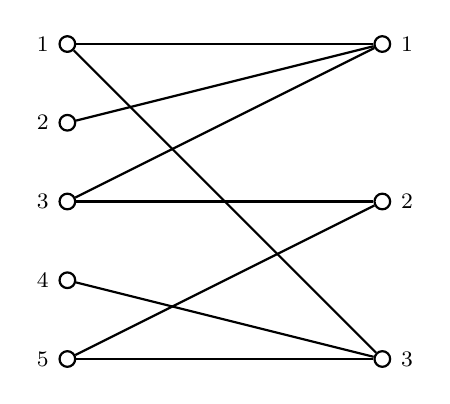
\begin{tikzpicture}
[lineDecorate/.style={-,thick},%
  nodeDecorate/.style={shape=circle,inner sep=2pt,draw,thick}]
%% nodes or vertices
\foreach \nodename/\nodelabel/\x/\y/\direction/\navigate in {
  c1/1/0/4/left/west, c2/2/0/3/left/west, c3/3/0/2/left/west,
  c4/4/0/1/left/west, c5/5/0/0/left/west, r1/1/4/4/right/east,
  r2/2/4/2/right/east, r3/3/4/0/right/east}
{
  \node (\nodename) at (\x,\y) [nodeDecorate] {};
  \node [\direction] at (\nodename.\navigate) {\footnotesize$\nodelabel$};
}
%% edges or lines
\path
\foreach \startnode/\endnode in {
  r1/c1, r1/c2, r1/c3, r2/c3, r2/c5, r3/c1, r3/c4, r3/c5}
{
  (\startnode) edge[lineDecorate] (\endnode)
};
\end{tikzpicture}
